\documentclass[twoside]{book}

% Packages required by doxygen
\usepackage{fixltx2e}
\usepackage{calc}
\usepackage{doxygen}
\usepackage[export]{adjustbox} % also loads graphicx
\usepackage{graphicx}
\usepackage[utf8]{inputenc}
\usepackage{makeidx}
\usepackage{multicol}
\usepackage{multirow}
\PassOptionsToPackage{warn}{textcomp}
\usepackage{textcomp}
\usepackage[nointegrals]{wasysym}
\usepackage[table]{xcolor}

% Font selection
\usepackage[T1]{fontenc}
\usepackage[scaled=.90]{helvet}
\usepackage{courier}
\usepackage{amssymb}
\usepackage{sectsty}
\renewcommand{\familydefault}{\sfdefault}
\allsectionsfont{%
  \fontseries{bc}\selectfont%
  \color{darkgray}%
}
\renewcommand{\DoxyLabelFont}{%
  \fontseries{bc}\selectfont%
  \color{darkgray}%
}
\newcommand{\+}{\discretionary{\mbox{\scriptsize$\hookleftarrow$}}{}{}}

% Page & text layout
\usepackage{geometry}
\geometry{%
  a4paper,%
  top=2.5cm,%
  bottom=2.5cm,%
  left=2.5cm,%
  right=2.5cm%
}
\tolerance=750
\hfuzz=15pt
\hbadness=750
\setlength{\emergencystretch}{15pt}
\setlength{\parindent}{0cm}
\setlength{\parskip}{0.2cm}
\makeatletter
\renewcommand{\paragraph}{%
  \@startsection{paragraph}{4}{0ex}{-1.0ex}{1.0ex}{%
    \normalfont\normalsize\bfseries\SS@parafont%
  }%
}
\renewcommand{\subparagraph}{%
  \@startsection{subparagraph}{5}{0ex}{-1.0ex}{1.0ex}{%
    \normalfont\normalsize\bfseries\SS@subparafont%
  }%
}
\makeatother

% Headers & footers
\usepackage{fancyhdr}
\pagestyle{fancyplain}
\fancyhead[LE]{\fancyplain{}{\bfseries\thepage}}
\fancyhead[CE]{\fancyplain{}{}}
\fancyhead[RE]{\fancyplain{}{\bfseries\leftmark}}
\fancyhead[LO]{\fancyplain{}{\bfseries\rightmark}}
\fancyhead[CO]{\fancyplain{}{}}
\fancyhead[RO]{\fancyplain{}{\bfseries\thepage}}
\fancyfoot[LE]{\fancyplain{}{}}
\fancyfoot[CE]{\fancyplain{}{}}
\fancyfoot[RE]{\fancyplain{}{\bfseries\scriptsize Generated on Mon Nov 16 2015 21\+:45\+:35 for Exercise Equipment Software by Doxygen }}
\fancyfoot[LO]{\fancyplain{}{\bfseries\scriptsize Generated on Mon Nov 16 2015 21\+:45\+:35 for Exercise Equipment Software by Doxygen }}
\fancyfoot[CO]{\fancyplain{}{}}
\fancyfoot[RO]{\fancyplain{}{}}
\renewcommand{\footrulewidth}{0.4pt}
\renewcommand{\chaptermark}[1]{%
  \markboth{#1}{}%
}
\renewcommand{\sectionmark}[1]{%
  \markright{\thesection\ #1}%
}

% Indices & bibliography
\usepackage{natbib}
\usepackage[titles]{tocloft}
\setcounter{tocdepth}{3}
\setcounter{secnumdepth}{5}
\makeindex

% Hyperlinks (required, but should be loaded last)
\usepackage{ifpdf}
\ifpdf
  \usepackage[pdftex,pagebackref=true]{hyperref}
\else
  \usepackage[ps2pdf,pagebackref=true]{hyperref}
\fi
\hypersetup{%
  colorlinks=true,%
  linkcolor=blue,%
  citecolor=blue,%
  unicode%
}

% Custom commands
\newcommand{\clearemptydoublepage}{%
  \newpage{\pagestyle{empty}\cleardoublepage}%
}


%===== C O N T E N T S =====

\begin{document}

% Titlepage & ToC
\hypersetup{pageanchor=false,
             bookmarks=true,
             bookmarksnumbered=true,
             pdfencoding=unicode
            }
\pagenumbering{roman}
\begin{titlepage}
\vspace*{7cm}
\begin{center}%
{\Large Exercise Equipment Software }\\
\vspace*{1cm}
{\large Generated by Doxygen 1.8.10}\\
\vspace*{0.5cm}
{\small Mon Nov 16 2015 21:45:35}\\
\end{center}
\end{titlepage}
\clearemptydoublepage
\tableofcontents
\clearemptydoublepage
\pagenumbering{arabic}
\hypersetup{pageanchor=true}

%--- Begin generated contents ---
\chapter{Hierarchical Index}
\section{Class Hierarchy}
This inheritance list is sorted roughly, but not completely, alphabetically\+:\begin{DoxyCompactList}
\item \contentsline{section}{Equipment\+Proto\+Factory}{\pageref{class_equipment_proto_factory}}{}
\item \contentsline{section}{Equipment\+Prototype}{\pageref{class_equipment_prototype}}{}
\begin{DoxyCompactList}
\item \contentsline{section}{Bike\+Prototype}{\pageref{class_bike_prototype}}{}
\item \contentsline{section}{Treadmill\+Prototype}{\pageref{class_treadmill_prototype}}{}
\end{DoxyCompactList}
\item Message\begin{DoxyCompactList}
\item \contentsline{section}{exercise\+\_\+protobuf\+:\+:Equipment}{\pageref{classexercise__protobuf_1_1_equipment}}{}
\item \contentsline{section}{exercise\+\_\+protobuf\+:\+:Gym}{\pageref{classexercise__protobuf_1_1_gym}}{}
\end{DoxyCompactList}
\item \contentsline{section}{Protobuf\+Interface}{\pageref{class_protobuf_interface}}{}
\item \contentsline{section}{exercise\+\_\+protobuf\+:\+:Static\+Descriptor\+Initializer\+\_\+exercise\+\_\+5fequipment\+\_\+2eproto}{\pageref{structexercise__protobuf_1_1_static_descriptor_initializer__exercise__5fequipment__2eproto}}{}
\end{DoxyCompactList}

\chapter{Class Index}
\section{Class List}
Here are the classes, structs, unions and interfaces with brief descriptions\+:\begin{DoxyCompactList}
\item\contentsline{section}{\hyperlink{class_bike_prototype}{Bike\+Prototype} \\*\hyperlink{class_bike_prototype}{Bike\+Prototype} Class }{\pageref{class_bike_prototype}}{}
\item\contentsline{section}{\hyperlink{classexercise__protobuf_1_1_equipment}{exercise\+\_\+protobuf\+::\+Equipment} }{\pageref{classexercise__protobuf_1_1_equipment}}{}
\item\contentsline{section}{\hyperlink{class_equipment_proto_factory}{Equipment\+Proto\+Factory} \\*\hyperlink{class_equipment_proto_factory}{Equipment\+Proto\+Factory} Class }{\pageref{class_equipment_proto_factory}}{}
\item\contentsline{section}{\hyperlink{class_equipment_prototype}{Equipment\+Prototype} \\*\hyperlink{class_equipment_prototype}{Equipment\+Prototype} Class }{\pageref{class_equipment_prototype}}{}
\item\contentsline{section}{\hyperlink{classexercise__protobuf_1_1_gym}{exercise\+\_\+protobuf\+::\+Gym} }{\pageref{classexercise__protobuf_1_1_gym}}{}
\item\contentsline{section}{\hyperlink{class_protobuf_interface}{Protobuf\+Interface} \\*\hyperlink{class_protobuf_interface}{Protobuf\+Interface} Class }{\pageref{class_protobuf_interface}}{}
\item\contentsline{section}{\hyperlink{structexercise__protobuf_1_1_static_descriptor_initializer__exercise__5fequipment__2eproto}{exercise\+\_\+protobuf\+::\+Static\+Descriptor\+Initializer\+\_\+exercise\+\_\+5fequipment\+\_\+2eproto} }{\pageref{structexercise__protobuf_1_1_static_descriptor_initializer__exercise__5fequipment__2eproto}}{}
\item\contentsline{section}{\hyperlink{class_treadmill_prototype}{Treadmill\+Prototype} \\*\hyperlink{class_treadmill_prototype}{Treadmill\+Prototype} Class }{\pageref{class_treadmill_prototype}}{}
\end{DoxyCompactList}

\chapter{Class Documentation}
\hypertarget{class_bike_prototype}{}\section{Bike\+Prototype Class Reference}
\label{class_bike_prototype}\index{Bike\+Prototype@{Bike\+Prototype}}


\hyperlink{class_bike_prototype}{Bike\+Prototype} Class.  




{\ttfamily \#include $<$bike\+\_\+prototype.\+hpp$>$}

Inheritance diagram for Bike\+Prototype\+:\begin{figure}[H]
\begin{center}
\leavevmode
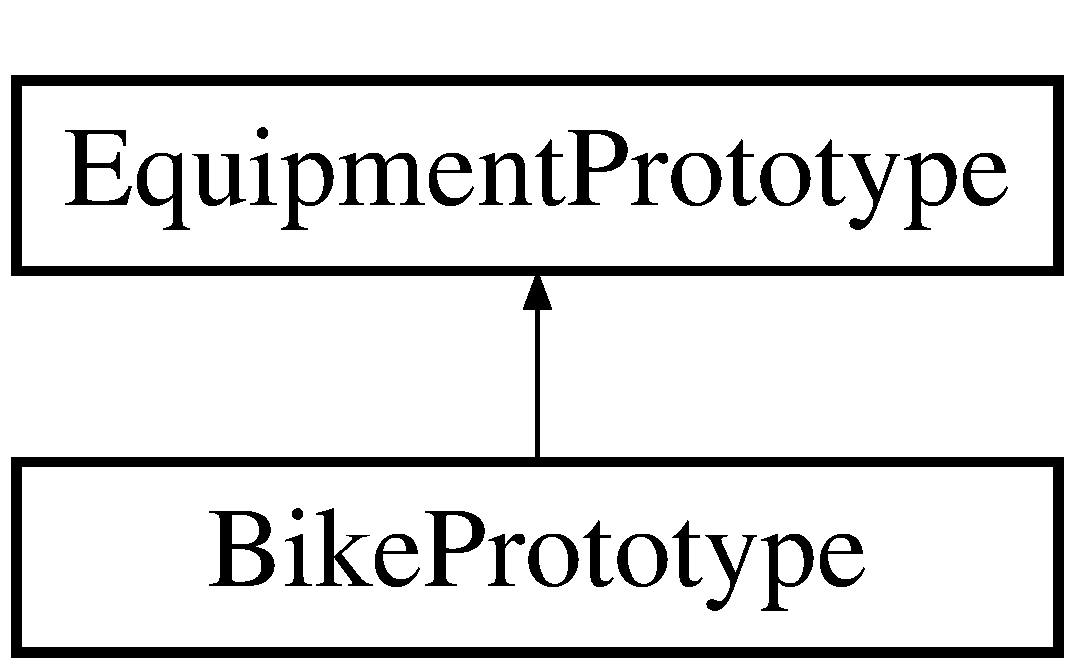
\includegraphics[height=2.000000cm]{class_bike_prototype}
\end{center}
\end{figure}
\subsection*{Public Member Functions}
\begin{DoxyCompactItemize}
\item 
\hypertarget{class_bike_prototype_ae49515bfb795c1a9000d7168fd764cc9}{}\hyperlink{class_bike_prototype_ae49515bfb795c1a9000d7168fd764cc9}{Bike\+Prototype} ()\label{class_bike_prototype_ae49515bfb795c1a9000d7168fd764cc9}

\begin{DoxyCompactList}\small\item\em Constructor. \end{DoxyCompactList}\item 
\hypertarget{class_bike_prototype_a044c34974541500ea818be723c65a64a}{}\hyperlink{class_bike_prototype_a044c34974541500ea818be723c65a64a}{Bike\+Prototype} (const \hyperlink{class_bike_prototype}{Bike\+Prototype} \&)\label{class_bike_prototype_a044c34974541500ea818be723c65a64a}

\begin{DoxyCompactList}\small\item\em Copy Constructor. \end{DoxyCompactList}\item 
\hyperlink{class_equipment_prototype}{Equipment\+Prototype} $\ast$ \hyperlink{class_bike_prototype_a10732d6849be44963b62994b724605b1}{clone} () const 
\begin{DoxyCompactList}\small\item\em Clone. \end{DoxyCompactList}\end{DoxyCompactItemize}
\subsection*{Additional Inherited Members}


\subsection{Detailed Description}
\hyperlink{class_bike_prototype}{Bike\+Prototype} Class. 

Used to hold information regarding an exercise bike. 

\subsection{Member Function Documentation}
\hypertarget{class_bike_prototype_a10732d6849be44963b62994b724605b1}{}\index{Bike\+Prototype@{Bike\+Prototype}!clone@{clone}}
\index{clone@{clone}!Bike\+Prototype@{Bike\+Prototype}}
\subsubsection[{clone() const }]{\setlength{\rightskip}{0pt plus 5cm}{\bf Equipment\+Prototype} $\ast$ Bike\+Prototype\+::clone (
\begin{DoxyParamCaption}
{}
\end{DoxyParamCaption}
) const\hspace{0.3cm}{\ttfamily [virtual]}}\label{class_bike_prototype_a10732d6849be44963b62994b724605b1}


Clone. 

Returns a new object that is identical to this one 

Implements \hyperlink{class_equipment_prototype_a4014d69b92c71c4c49477c657c824024}{Equipment\+Prototype}.



The documentation for this class was generated from the following files\+:\begin{DoxyCompactItemize}
\item 
/\+Users/jshier/\+Development/\+Exercise\+Software/\+Exercise\+Software/bike\+\_\+prototype.\+hpp\item 
/\+Users/jshier/\+Development/\+Exercise\+Software/\+Exercise\+Software/bike\+\_\+prototype.\+cpp\end{DoxyCompactItemize}

\hypertarget{classexercise__protobuf_1_1_equipment}{}\section{exercise\+\_\+protobuf\+:\+:Equipment Class Reference}
\label{classexercise__protobuf_1_1_equipment}\index{exercise\+\_\+protobuf\+::\+Equipment@{exercise\+\_\+protobuf\+::\+Equipment}}
Inheritance diagram for exercise\+\_\+protobuf\+:\+:Equipment\+:\begin{figure}[H]
\begin{center}
\leavevmode
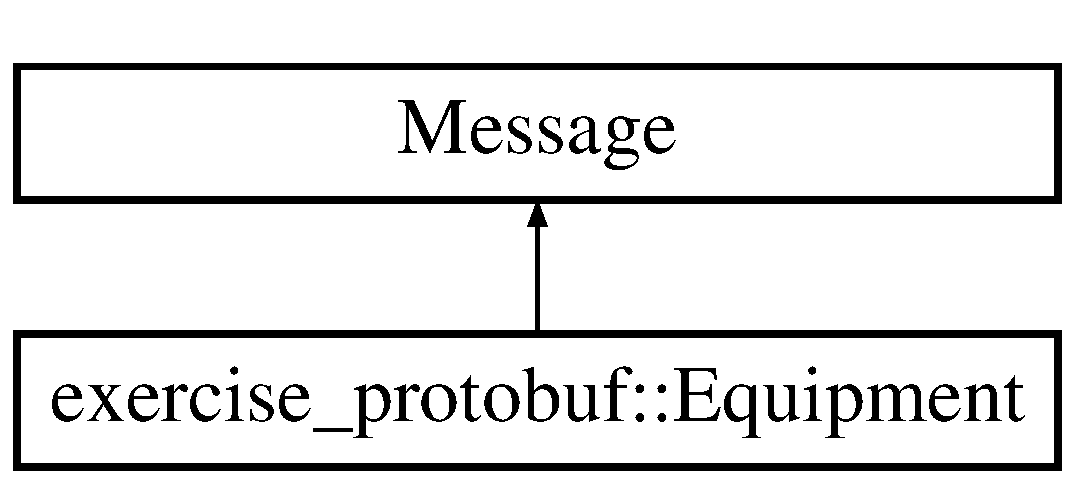
\includegraphics[height=2.000000cm]{classexercise__protobuf_1_1_equipment}
\end{center}
\end{figure}
\subsection*{Public Member Functions}
\begin{DoxyCompactItemize}
\item 
\hypertarget{classexercise__protobuf_1_1_equipment_a15a46b44fbeb733ae519e0168c83b09e}{}{\bfseries Equipment} (const \hyperlink{classexercise__protobuf_1_1_equipment}{Equipment} \&from)\label{classexercise__protobuf_1_1_equipment_a15a46b44fbeb733ae519e0168c83b09e}

\item 
\hypertarget{classexercise__protobuf_1_1_equipment_a5f2af2e5770332e1c06b32113c5f9f1d}{}\hyperlink{classexercise__protobuf_1_1_equipment}{Equipment} \& {\bfseries operator=} (const \hyperlink{classexercise__protobuf_1_1_equipment}{Equipment} \&from)\label{classexercise__protobuf_1_1_equipment_a5f2af2e5770332e1c06b32113c5f9f1d}

\item 
\hypertarget{classexercise__protobuf_1_1_equipment_ac5015943deab60d649526b752273d169}{}const \+::google\+::protobuf\+::\+Unknown\+Field\+Set \& {\bfseries unknown\+\_\+fields} () const \label{classexercise__protobuf_1_1_equipment_ac5015943deab60d649526b752273d169}

\item 
\hypertarget{classexercise__protobuf_1_1_equipment_a3bce73a5183112dc976709f2bbfe820c}{}inline\+::google\+::protobuf\+::\+Unknown\+Field\+Set $\ast$ {\bfseries mutable\+\_\+unknown\+\_\+fields} ()\label{classexercise__protobuf_1_1_equipment_a3bce73a5183112dc976709f2bbfe820c}

\item 
\hypertarget{classexercise__protobuf_1_1_equipment_af7393bf7eaa3be2e73c3d251ba29842a}{}void {\bfseries Swap} (\hyperlink{classexercise__protobuf_1_1_equipment}{Equipment} $\ast$other)\label{classexercise__protobuf_1_1_equipment_af7393bf7eaa3be2e73c3d251ba29842a}

\item 
\hypertarget{classexercise__protobuf_1_1_equipment_ad63093acbdcc73dcc1f584a1779517b8}{}\hyperlink{classexercise__protobuf_1_1_equipment}{Equipment} $\ast$ {\bfseries New} () const \label{classexercise__protobuf_1_1_equipment_ad63093acbdcc73dcc1f584a1779517b8}

\item 
\hypertarget{classexercise__protobuf_1_1_equipment_a8e35d1a0ea5bb7f51b7ad786040f2fc3}{}void {\bfseries Copy\+From} (const \+::google\+::protobuf\+::\+Message \&from)\label{classexercise__protobuf_1_1_equipment_a8e35d1a0ea5bb7f51b7ad786040f2fc3}

\item 
\hypertarget{classexercise__protobuf_1_1_equipment_a6e4ae455cebc693ad0c1d39163929ab1}{}void {\bfseries Merge\+From} (const \+::google\+::protobuf\+::\+Message \&from)\label{classexercise__protobuf_1_1_equipment_a6e4ae455cebc693ad0c1d39163929ab1}

\item 
\hypertarget{classexercise__protobuf_1_1_equipment_a512c709e77a5f1d15426dd99e0ce4a9e}{}void {\bfseries Copy\+From} (const \hyperlink{classexercise__protobuf_1_1_equipment}{Equipment} \&from)\label{classexercise__protobuf_1_1_equipment_a512c709e77a5f1d15426dd99e0ce4a9e}

\item 
\hypertarget{classexercise__protobuf_1_1_equipment_a0c19672b9b434ac5c4da0b6aa60babec}{}void {\bfseries Merge\+From} (const \hyperlink{classexercise__protobuf_1_1_equipment}{Equipment} \&from)\label{classexercise__protobuf_1_1_equipment_a0c19672b9b434ac5c4da0b6aa60babec}

\item 
\hypertarget{classexercise__protobuf_1_1_equipment_a9d086db65d11324fd1591b532e3046ba}{}void {\bfseries Clear} ()\label{classexercise__protobuf_1_1_equipment_a9d086db65d11324fd1591b532e3046ba}

\item 
\hypertarget{classexercise__protobuf_1_1_equipment_ad1c0086ae587c1ec120aa3ee2ed24a26}{}bool {\bfseries Is\+Initialized} () const \label{classexercise__protobuf_1_1_equipment_ad1c0086ae587c1ec120aa3ee2ed24a26}

\item 
\hypertarget{classexercise__protobuf_1_1_equipment_a96fd0e95500177cd9da1e47fe30bec33}{}int {\bfseries Byte\+Size} () const \label{classexercise__protobuf_1_1_equipment_a96fd0e95500177cd9da1e47fe30bec33}

\item 
\hypertarget{classexercise__protobuf_1_1_equipment_ad9774ec88526a3f393566233b399ffab}{}bool {\bfseries Merge\+Partial\+From\+Coded\+Stream} (\+::google\+::protobuf\+::io\+::\+Coded\+Input\+Stream $\ast$input)\label{classexercise__protobuf_1_1_equipment_ad9774ec88526a3f393566233b399ffab}

\item 
\hypertarget{classexercise__protobuf_1_1_equipment_afcb7d68b3a7a3523f87a31833f235189}{}void {\bfseries Serialize\+With\+Cached\+Sizes} (\+::google\+::protobuf\+::io\+::\+Coded\+Output\+Stream $\ast$output) const \label{classexercise__protobuf_1_1_equipment_afcb7d68b3a7a3523f87a31833f235189}

\item 
\hypertarget{classexercise__protobuf_1_1_equipment_a01b12466e3bca65be96dfe1137c11678}{}\+::google\+::protobuf\+::uint8 $\ast$ {\bfseries Serialize\+With\+Cached\+Sizes\+To\+Array} (\+::google\+::protobuf\+::uint8 $\ast$output) const \label{classexercise__protobuf_1_1_equipment_a01b12466e3bca65be96dfe1137c11678}

\item 
\hypertarget{classexercise__protobuf_1_1_equipment_af54af5e38428b24a8094c9e86218be83}{}int {\bfseries Get\+Cached\+Size} () const \label{classexercise__protobuf_1_1_equipment_af54af5e38428b24a8094c9e86218be83}

\item 
\hypertarget{classexercise__protobuf_1_1_equipment_a7594133c99cde742d22d00c4854833da}{}\+::google\+::protobuf\+::\+Metadata {\bfseries Get\+Metadata} () const \label{classexercise__protobuf_1_1_equipment_a7594133c99cde742d22d00c4854833da}

\item 
\hypertarget{classexercise__protobuf_1_1_equipment_ad6e3390388ee6ace059a8f5e9a76aff1}{}bool {\bfseries has\+\_\+id} () const \label{classexercise__protobuf_1_1_equipment_ad6e3390388ee6ace059a8f5e9a76aff1}

\item 
\hypertarget{classexercise__protobuf_1_1_equipment_aa020e32b0f5ce92f65acc5d60905cd26}{}void {\bfseries clear\+\_\+id} ()\label{classexercise__protobuf_1_1_equipment_aa020e32b0f5ce92f65acc5d60905cd26}

\item 
\hypertarget{classexercise__protobuf_1_1_equipment_abf5f9c64761ec799143e120f56334fdc}{}inline\+::google\+::protobuf\+::int32 {\bfseries id} () const \label{classexercise__protobuf_1_1_equipment_abf5f9c64761ec799143e120f56334fdc}

\item 
\hypertarget{classexercise__protobuf_1_1_equipment_ac488d786fe74db48c938adae4255b400}{}void {\bfseries set\+\_\+id} (\+::google\+::protobuf\+::int32 value)\label{classexercise__protobuf_1_1_equipment_ac488d786fe74db48c938adae4255b400}

\item 
\hypertarget{classexercise__protobuf_1_1_equipment_a0dcc73af1c1261c194df9d3635df4228}{}bool {\bfseries has\+\_\+type} () const \label{classexercise__protobuf_1_1_equipment_a0dcc73af1c1261c194df9d3635df4228}

\item 
\hypertarget{classexercise__protobuf_1_1_equipment_a2d631bc102d777cc06b3db458461ad65}{}void {\bfseries clear\+\_\+type} ()\label{classexercise__protobuf_1_1_equipment_a2d631bc102d777cc06b3db458461ad65}

\item 
\hypertarget{classexercise__protobuf_1_1_equipment_a9a17d01d878722c16bc41df77b03f075}{}const \+::std\+::string \& {\bfseries type} () const \label{classexercise__protobuf_1_1_equipment_a9a17d01d878722c16bc41df77b03f075}

\item 
\hypertarget{classexercise__protobuf_1_1_equipment_af17c050a48f9d33187c6326a5c6a73c4}{}void {\bfseries set\+\_\+type} (const \+::std\+::string \&value)\label{classexercise__protobuf_1_1_equipment_af17c050a48f9d33187c6326a5c6a73c4}

\item 
\hypertarget{classexercise__protobuf_1_1_equipment_a8ad4e6ef135e301a95549807d862d0e9}{}void {\bfseries set\+\_\+type} (const char $\ast$value)\label{classexercise__protobuf_1_1_equipment_a8ad4e6ef135e301a95549807d862d0e9}

\item 
\hypertarget{classexercise__protobuf_1_1_equipment_adce77f3b469621ebefbb6ccd93ca08fc}{}void {\bfseries set\+\_\+type} (const char $\ast$value, size\+\_\+t size)\label{classexercise__protobuf_1_1_equipment_adce77f3b469621ebefbb6ccd93ca08fc}

\item 
\hypertarget{classexercise__protobuf_1_1_equipment_a168312a2203f7ac090d5b4282bf468af}{}inline\+::std\+::string $\ast$ {\bfseries mutable\+\_\+type} ()\label{classexercise__protobuf_1_1_equipment_a168312a2203f7ac090d5b4282bf468af}

\item 
\hypertarget{classexercise__protobuf_1_1_equipment_a027d7ccf12f075f7a004b6e048a40da0}{}inline\+::std\+::string $\ast$ {\bfseries release\+\_\+type} ()\label{classexercise__protobuf_1_1_equipment_a027d7ccf12f075f7a004b6e048a40da0}

\item 
\hypertarget{classexercise__protobuf_1_1_equipment_a4eaedfe6e67f8ad131d4eb14804b95fe}{}void {\bfseries set\+\_\+allocated\+\_\+type} (\+::std\+::string $\ast$type)\label{classexercise__protobuf_1_1_equipment_a4eaedfe6e67f8ad131d4eb14804b95fe}

\end{DoxyCompactItemize}
\subsection*{Static Public Member Functions}
\begin{DoxyCompactItemize}
\item 
\hypertarget{classexercise__protobuf_1_1_equipment_a2f38981061fdada40a9249d6fd91a61b}{}static const \+::google\+::protobuf\+::\+Descriptor $\ast$ {\bfseries descriptor} ()\label{classexercise__protobuf_1_1_equipment_a2f38981061fdada40a9249d6fd91a61b}

\item 
\hypertarget{classexercise__protobuf_1_1_equipment_a9a202a511ef35f8e584ae395553446b6}{}static const \hyperlink{classexercise__protobuf_1_1_equipment}{Equipment} \& {\bfseries default\+\_\+instance} ()\label{classexercise__protobuf_1_1_equipment_a9a202a511ef35f8e584ae395553446b6}

\end{DoxyCompactItemize}
\subsection*{Static Public Attributes}
\begin{DoxyCompactItemize}
\item 
\hypertarget{classexercise__protobuf_1_1_equipment_a5e646568504125c15d9e7097aa061c9e}{}static const int {\bfseries k\+Id\+Field\+Number} = 1\label{classexercise__protobuf_1_1_equipment_a5e646568504125c15d9e7097aa061c9e}

\item 
\hypertarget{classexercise__protobuf_1_1_equipment_a3c28ba0b445abab11d6a6c948d622a1c}{}static const int {\bfseries k\+Type\+Field\+Number} = 2\label{classexercise__protobuf_1_1_equipment_a3c28ba0b445abab11d6a6c948d622a1c}

\end{DoxyCompactItemize}
\subsection*{Friends}
\begin{DoxyCompactItemize}
\item 
\hypertarget{classexercise__protobuf_1_1_equipment_ab643513d59abee7e930172a51104e178}{}void {\bfseries protobuf\+\_\+\+Add\+Desc\+\_\+exercise\+\_\+5fequipment\+\_\+2eproto} ()\label{classexercise__protobuf_1_1_equipment_ab643513d59abee7e930172a51104e178}

\item 
\hypertarget{classexercise__protobuf_1_1_equipment_aa2ddf289362adb3ea15b10dee7c74676}{}void {\bfseries protobuf\+\_\+\+Assign\+Desc\+\_\+exercise\+\_\+5fequipment\+\_\+2eproto} ()\label{classexercise__protobuf_1_1_equipment_aa2ddf289362adb3ea15b10dee7c74676}

\item 
\hypertarget{classexercise__protobuf_1_1_equipment_a04b681f62a7ad9cafa043f7d5a95e743}{}void {\bfseries protobuf\+\_\+\+Shutdown\+File\+\_\+exercise\+\_\+5fequipment\+\_\+2eproto} ()\label{classexercise__protobuf_1_1_equipment_a04b681f62a7ad9cafa043f7d5a95e743}

\end{DoxyCompactItemize}


The documentation for this class was generated from the following files\+:\begin{DoxyCompactItemize}
\item 
/\+Users/jshier/\+Development/\+Exercise\+Software/\+Exercise\+Software/exercise\+\_\+equipment.\+pb.\+h\item 
/\+Users/jshier/\+Development/\+Exercise\+Software/\+Exercise\+Software/exercise\+\_\+equipment.\+pb.\+cc\end{DoxyCompactItemize}

\hypertarget{class_equipment_proto_factory}{}\section{Equipment\+Proto\+Factory Class Reference}
\label{class_equipment_proto_factory}\index{Equipment\+Proto\+Factory@{Equipment\+Proto\+Factory}}


\hyperlink{class_equipment_proto_factory}{Equipment\+Proto\+Factory} Class.  




{\ttfamily \#include $<$equipment\+\_\+proto\+\_\+factory.\+hpp$>$}

\subsection*{Public Member Functions}
\begin{DoxyCompactItemize}
\item 
\hypertarget{class_equipment_proto_factory_aa5d0da8b143ac289d645a22b26c37569}{}\hyperlink{class_equipment_proto_factory_aa5d0da8b143ac289d645a22b26c37569}{Equipment\+Proto\+Factory} ()\label{class_equipment_proto_factory_aa5d0da8b143ac289d645a22b26c37569}

\begin{DoxyCompactList}\small\item\em Constructor. \end{DoxyCompactList}\item 
\hypertarget{class_equipment_proto_factory_ad33d994f3281f492aaa3cd305889f780}{}\hyperlink{class_equipment_proto_factory_ad33d994f3281f492aaa3cd305889f780}{$\sim$\+Equipment\+Proto\+Factory} ()\label{class_equipment_proto_factory_ad33d994f3281f492aaa3cd305889f780}

\begin{DoxyCompactList}\small\item\em Destructor. \end{DoxyCompactList}\item 
\hypertarget{class_equipment_proto_factory_a18e0b0214b22722e59f80fef954da6e7}{}\hyperlink{class_equipment_prototype}{Equipment\+Prototype} $\ast$ \hyperlink{class_equipment_proto_factory_a18e0b0214b22722e59f80fef954da6e7}{get\+Equipment} (enum Equipment\+Type)\label{class_equipment_proto_factory_a18e0b0214b22722e59f80fef954da6e7}

\begin{DoxyCompactList}\small\item\em Returns a new \hyperlink{class_equipment_prototype}{Equipment\+Prototype} object of the type requested. \end{DoxyCompactList}\item 
\hypertarget{class_equipment_proto_factory_adccf993cd9070d41d4907bd6c8acb6c8}{}Equipment\+Type \hyperlink{class_equipment_proto_factory_adccf993cd9070d41d4907bd6c8acb6c8}{get\+Equipment\+Type} (std\+::string)\label{class_equipment_proto_factory_adccf993cd9070d41d4907bd6c8acb6c8}

\begin{DoxyCompactList}\small\item\em Maps a string of an equipment type to the enum\+: Equipment\+Type. \end{DoxyCompactList}\item 
\hypertarget{class_equipment_proto_factory_a85965709ee05ef53303c9448b35aea60}{}std\+::string \hyperlink{class_equipment_proto_factory_a85965709ee05ef53303c9448b35aea60}{get\+Types} ()\label{class_equipment_proto_factory_a85965709ee05ef53303c9448b35aea60}

\begin{DoxyCompactList}\small\item\em Get a list of types of equipment available for selection. \end{DoxyCompactList}\end{DoxyCompactItemize}


\subsection{Detailed Description}
\hyperlink{class_equipment_proto_factory}{Equipment\+Proto\+Factory} Class. 

Factory class for getting new equipment prototype objects of a particular type 

The documentation for this class was generated from the following files\+:\begin{DoxyCompactItemize}
\item 
/\+Users/jshier/\+Development/\+Exercise\+Software/\+Exercise\+Software/equipment\+\_\+proto\+\_\+factory.\+hpp\item 
/\+Users/jshier/\+Development/\+Exercise\+Software/\+Exercise\+Software/equipment\+\_\+proto\+\_\+factory.\+cpp\end{DoxyCompactItemize}

\hypertarget{class_equipment_prototype}{}\section{Equipment\+Prototype Class Reference}
\label{class_equipment_prototype}\index{Equipment\+Prototype@{Equipment\+Prototype}}


\hyperlink{class_equipment_prototype}{Equipment\+Prototype} Class.  




{\ttfamily \#include $<$equipment\+\_\+prototype.\+hpp$>$}

Inheritance diagram for Equipment\+Prototype\+:\begin{figure}[H]
\begin{center}
\leavevmode
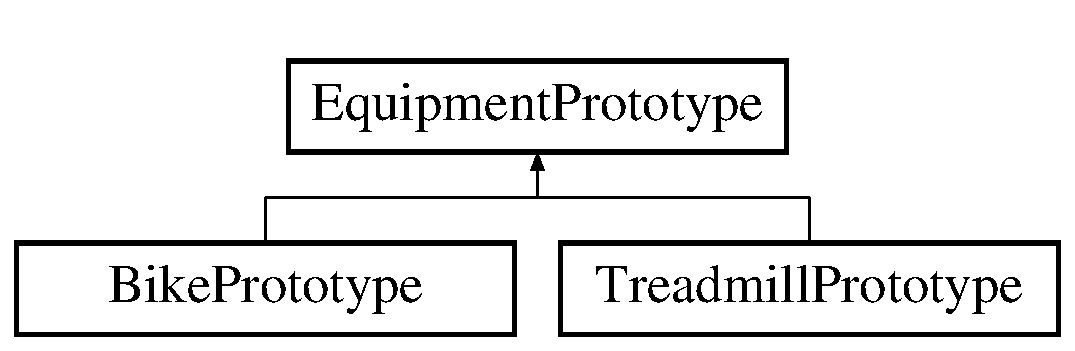
\includegraphics[height=2.000000cm]{class_equipment_prototype}
\end{center}
\end{figure}
\subsection*{Public Member Functions}
\begin{DoxyCompactItemize}
\item 
virtual \hyperlink{class_equipment_prototype}{Equipment\+Prototype} $\ast$ \hyperlink{class_equipment_prototype_a4014d69b92c71c4c49477c657c824024}{clone} () const  =0
\begin{DoxyCompactList}\small\item\em Clone. \end{DoxyCompactList}\item 
\hypertarget{class_equipment_prototype_aab050a04930f86328433401e7ad2d589}{}virtual void \hyperlink{class_equipment_prototype_aab050a04930f86328433401e7ad2d589}{set\+Type} (std\+::string)\label{class_equipment_prototype_aab050a04930f86328433401e7ad2d589}

\begin{DoxyCompactList}\small\item\em Set the type of this equipment. \end{DoxyCompactList}\item 
\hypertarget{class_equipment_prototype_af165565c75afeb2c4a214cb6dd2209b6}{}virtual std\+::string \hyperlink{class_equipment_prototype_af165565c75afeb2c4a214cb6dd2209b6}{get\+Type} () const \label{class_equipment_prototype_af165565c75afeb2c4a214cb6dd2209b6}

\begin{DoxyCompactList}\small\item\em Get the type of this equipment. \end{DoxyCompactList}\item 
\hypertarget{class_equipment_prototype_accf753d12a43903655f45baea8343f5a}{}virtual void \hyperlink{class_equipment_prototype_accf753d12a43903655f45baea8343f5a}{set\+Id} (int)\label{class_equipment_prototype_accf753d12a43903655f45baea8343f5a}

\begin{DoxyCompactList}\small\item\em Set the id of this equipment. \end{DoxyCompactList}\item 
\hypertarget{class_equipment_prototype_af34187c2a2552f0d6ee30de69a4b1a59}{}virtual int \hyperlink{class_equipment_prototype_af34187c2a2552f0d6ee30de69a4b1a59}{get\+Id} () const \label{class_equipment_prototype_af34187c2a2552f0d6ee30de69a4b1a59}

\begin{DoxyCompactList}\small\item\em Get the id value for this equipment. \end{DoxyCompactList}\end{DoxyCompactItemize}
\subsection*{Protected Attributes}
\begin{DoxyCompactItemize}
\item 
\hypertarget{class_equipment_prototype_a3fc27f367f2950fbe0d5b82c9224ffa2}{}int \hyperlink{class_equipment_prototype_a3fc27f367f2950fbe0d5b82c9224ffa2}{\+\_\+id}\label{class_equipment_prototype_a3fc27f367f2950fbe0d5b82c9224ffa2}

\begin{DoxyCompactList}\small\item\em Unique I\+D value of equipment. \end{DoxyCompactList}\item 
\hypertarget{class_equipment_prototype_a001dba508f99f42521b8ada235783645}{}std\+::string \hyperlink{class_equipment_prototype_a001dba508f99f42521b8ada235783645}{\+\_\+type}\label{class_equipment_prototype_a001dba508f99f42521b8ada235783645}

\begin{DoxyCompactList}\small\item\em Type of equipment being represented. \end{DoxyCompactList}\end{DoxyCompactItemize}


\subsection{Detailed Description}
\hyperlink{class_equipment_prototype}{Equipment\+Prototype} Class. 

Abstract Base Class for all Equipment Classes 

\subsection{Member Function Documentation}
\hypertarget{class_equipment_prototype_a4014d69b92c71c4c49477c657c824024}{}\index{Equipment\+Prototype@{Equipment\+Prototype}!clone@{clone}}
\index{clone@{clone}!Equipment\+Prototype@{Equipment\+Prototype}}
\subsubsection[{clone() const  =0}]{\setlength{\rightskip}{0pt plus 5cm}virtual {\bf Equipment\+Prototype}$\ast$ Equipment\+Prototype\+::clone (
\begin{DoxyParamCaption}
{}
\end{DoxyParamCaption}
) const\hspace{0.3cm}{\ttfamily [pure virtual]}}\label{class_equipment_prototype_a4014d69b92c71c4c49477c657c824024}


Clone. 

Must be overriden in child class 

Implemented in \hyperlink{class_treadmill_prototype_abd7e7f894721af9f03b248b6617d4fdc}{Treadmill\+Prototype}, and \hyperlink{class_bike_prototype_a10732d6849be44963b62994b724605b1}{Bike\+Prototype}.



The documentation for this class was generated from the following files\+:\begin{DoxyCompactItemize}
\item 
/\+Users/jshier/\+Development/\+Exercise\+Software/\+Exercise\+Software/equipment\+\_\+prototype.\+hpp\item 
/\+Users/jshier/\+Development/\+Exercise\+Software/\+Exercise\+Software/equipment\+\_\+prototype.\+cpp\end{DoxyCompactItemize}

\hypertarget{classexercise__protobuf_1_1_gym}{}\section{exercise\+\_\+protobuf\+:\+:Gym Class Reference}
\label{classexercise__protobuf_1_1_gym}\index{exercise\+\_\+protobuf\+::\+Gym@{exercise\+\_\+protobuf\+::\+Gym}}
Inheritance diagram for exercise\+\_\+protobuf\+:\+:Gym\+:\begin{figure}[H]
\begin{center}
\leavevmode
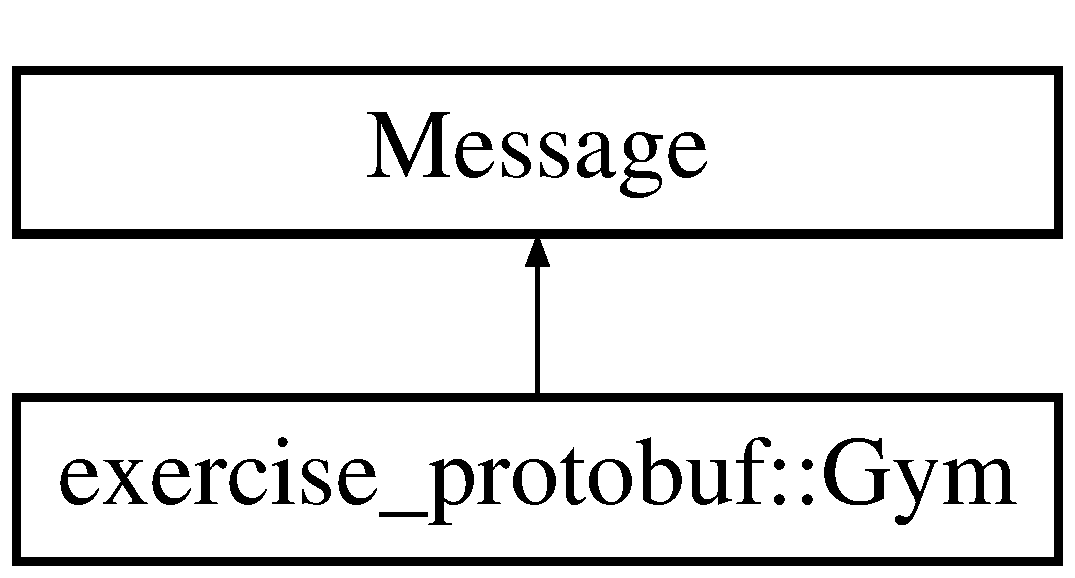
\includegraphics[height=2.000000cm]{classexercise__protobuf_1_1_gym}
\end{center}
\end{figure}
\subsection*{Public Member Functions}
\begin{DoxyCompactItemize}
\item 
\hypertarget{classexercise__protobuf_1_1_gym_aedf540820ea28179f800019a5d2878e7}{}{\bfseries Gym} (const \hyperlink{classexercise__protobuf_1_1_gym}{Gym} \&from)\label{classexercise__protobuf_1_1_gym_aedf540820ea28179f800019a5d2878e7}

\item 
\hypertarget{classexercise__protobuf_1_1_gym_aa445fc51b8f08f6f955c584986cb786c}{}\hyperlink{classexercise__protobuf_1_1_gym}{Gym} \& {\bfseries operator=} (const \hyperlink{classexercise__protobuf_1_1_gym}{Gym} \&from)\label{classexercise__protobuf_1_1_gym_aa445fc51b8f08f6f955c584986cb786c}

\item 
\hypertarget{classexercise__protobuf_1_1_gym_a95b77c95cb7b94d13b5dd0bc06975476}{}const \+::google\+::protobuf\+::\+Unknown\+Field\+Set \& {\bfseries unknown\+\_\+fields} () const \label{classexercise__protobuf_1_1_gym_a95b77c95cb7b94d13b5dd0bc06975476}

\item 
\hypertarget{classexercise__protobuf_1_1_gym_a5c9ac1981c2183dff6c888c3364d8bee}{}inline\+::google\+::protobuf\+::\+Unknown\+Field\+Set $\ast$ {\bfseries mutable\+\_\+unknown\+\_\+fields} ()\label{classexercise__protobuf_1_1_gym_a5c9ac1981c2183dff6c888c3364d8bee}

\item 
\hypertarget{classexercise__protobuf_1_1_gym_abf56c14bbf7c0bac857af6743f19ab97}{}void {\bfseries Swap} (\hyperlink{classexercise__protobuf_1_1_gym}{Gym} $\ast$other)\label{classexercise__protobuf_1_1_gym_abf56c14bbf7c0bac857af6743f19ab97}

\item 
\hypertarget{classexercise__protobuf_1_1_gym_a376d416d53df49a87de25d62a40526ea}{}\hyperlink{classexercise__protobuf_1_1_gym}{Gym} $\ast$ {\bfseries New} () const \label{classexercise__protobuf_1_1_gym_a376d416d53df49a87de25d62a40526ea}

\item 
\hypertarget{classexercise__protobuf_1_1_gym_a7094f8391d1ed49797dac887057f4825}{}void {\bfseries Copy\+From} (const \+::google\+::protobuf\+::\+Message \&from)\label{classexercise__protobuf_1_1_gym_a7094f8391d1ed49797dac887057f4825}

\item 
\hypertarget{classexercise__protobuf_1_1_gym_afd460c91ffe194457fd04db10cb7bd8a}{}void {\bfseries Merge\+From} (const \+::google\+::protobuf\+::\+Message \&from)\label{classexercise__protobuf_1_1_gym_afd460c91ffe194457fd04db10cb7bd8a}

\item 
\hypertarget{classexercise__protobuf_1_1_gym_aba20cab66b8d8b8ba595dcee442be7b5}{}void {\bfseries Copy\+From} (const \hyperlink{classexercise__protobuf_1_1_gym}{Gym} \&from)\label{classexercise__protobuf_1_1_gym_aba20cab66b8d8b8ba595dcee442be7b5}

\item 
\hypertarget{classexercise__protobuf_1_1_gym_a73546f80d8e0922b723364bd3204919d}{}void {\bfseries Merge\+From} (const \hyperlink{classexercise__protobuf_1_1_gym}{Gym} \&from)\label{classexercise__protobuf_1_1_gym_a73546f80d8e0922b723364bd3204919d}

\item 
\hypertarget{classexercise__protobuf_1_1_gym_a852de6c227b4bbaf74f666d1837eec1a}{}void {\bfseries Clear} ()\label{classexercise__protobuf_1_1_gym_a852de6c227b4bbaf74f666d1837eec1a}

\item 
\hypertarget{classexercise__protobuf_1_1_gym_a79104f16342a99edf1141466cfebc8be}{}bool {\bfseries Is\+Initialized} () const \label{classexercise__protobuf_1_1_gym_a79104f16342a99edf1141466cfebc8be}

\item 
\hypertarget{classexercise__protobuf_1_1_gym_a886e7dab292a3d10f47d6d1891f72973}{}int {\bfseries Byte\+Size} () const \label{classexercise__protobuf_1_1_gym_a886e7dab292a3d10f47d6d1891f72973}

\item 
\hypertarget{classexercise__protobuf_1_1_gym_abc70c5b2303f2bd5fa41740d5f81a528}{}bool {\bfseries Merge\+Partial\+From\+Coded\+Stream} (\+::google\+::protobuf\+::io\+::\+Coded\+Input\+Stream $\ast$input)\label{classexercise__protobuf_1_1_gym_abc70c5b2303f2bd5fa41740d5f81a528}

\item 
\hypertarget{classexercise__protobuf_1_1_gym_a5f0ce954d508579596f36db637a0a130}{}void {\bfseries Serialize\+With\+Cached\+Sizes} (\+::google\+::protobuf\+::io\+::\+Coded\+Output\+Stream $\ast$output) const \label{classexercise__protobuf_1_1_gym_a5f0ce954d508579596f36db637a0a130}

\item 
\hypertarget{classexercise__protobuf_1_1_gym_a283d77c471e32f05d155112ecf2d1998}{}\+::google\+::protobuf\+::uint8 $\ast$ {\bfseries Serialize\+With\+Cached\+Sizes\+To\+Array} (\+::google\+::protobuf\+::uint8 $\ast$output) const \label{classexercise__protobuf_1_1_gym_a283d77c471e32f05d155112ecf2d1998}

\item 
\hypertarget{classexercise__protobuf_1_1_gym_a48ffc8148ee8dae3cf0c6dc30c84bd55}{}int {\bfseries Get\+Cached\+Size} () const \label{classexercise__protobuf_1_1_gym_a48ffc8148ee8dae3cf0c6dc30c84bd55}

\item 
\hypertarget{classexercise__protobuf_1_1_gym_a4760b64829ff017c841ce2ee358c2d01}{}\+::google\+::protobuf\+::\+Metadata {\bfseries Get\+Metadata} () const \label{classexercise__protobuf_1_1_gym_a4760b64829ff017c841ce2ee358c2d01}

\item 
\hypertarget{classexercise__protobuf_1_1_gym_a27a4f396faff45ce740c2e97fc607af4}{}int {\bfseries equipment\+\_\+size} () const \label{classexercise__protobuf_1_1_gym_a27a4f396faff45ce740c2e97fc607af4}

\item 
\hypertarget{classexercise__protobuf_1_1_gym_a39fd155db773fdeeb782acac7fc540e0}{}void {\bfseries clear\+\_\+equipment} ()\label{classexercise__protobuf_1_1_gym_a39fd155db773fdeeb782acac7fc540e0}

\item 
\hypertarget{classexercise__protobuf_1_1_gym_abf15a9b9acc08a0404fe4c8f0c0b1992}{}const \+::\hyperlink{classexercise__protobuf_1_1_equipment}{exercise\+\_\+protobuf\+::\+Equipment} \& {\bfseries equipment} (int index) const \label{classexercise__protobuf_1_1_gym_abf15a9b9acc08a0404fe4c8f0c0b1992}

\item 
\hypertarget{classexercise__protobuf_1_1_gym_aa5082078c89fd294ea528c85068fab44}{}inline\+::exercise\+\_\+protobuf\+::\+Equipment $\ast$ {\bfseries mutable\+\_\+equipment} (int index)\label{classexercise__protobuf_1_1_gym_aa5082078c89fd294ea528c85068fab44}

\item 
\hypertarget{classexercise__protobuf_1_1_gym_a627f83620cd7153b868239224731a1ee}{}inline\+::exercise\+\_\+protobuf\+::\+Equipment $\ast$ {\bfseries add\+\_\+equipment} ()\label{classexercise__protobuf_1_1_gym_a627f83620cd7153b868239224731a1ee}

\item 
\hypertarget{classexercise__protobuf_1_1_gym_a8e34caf50624d20ec7842667c094ec84}{}const \+::google\+::protobuf\+::\+Repeated\+Ptr\+Field$<$ \+::\hyperlink{classexercise__protobuf_1_1_equipment}{exercise\+\_\+protobuf\+::\+Equipment} $>$ \& {\bfseries equipment} () const \label{classexercise__protobuf_1_1_gym_a8e34caf50624d20ec7842667c094ec84}

\item 
\hypertarget{classexercise__protobuf_1_1_gym_a69c1805ad995d89710319b12efd1cf94}{}inline\+::google\+::protobuf\+::\+Repeated\+Ptr\+Field$<$ \+::\hyperlink{classexercise__protobuf_1_1_equipment}{exercise\+\_\+protobuf\+::\+Equipment} $>$ $\ast$ {\bfseries mutable\+\_\+equipment} ()\label{classexercise__protobuf_1_1_gym_a69c1805ad995d89710319b12efd1cf94}

\end{DoxyCompactItemize}
\subsection*{Static Public Member Functions}
\begin{DoxyCompactItemize}
\item 
\hypertarget{classexercise__protobuf_1_1_gym_ac3a0e2edcb27d960aa09da71d74f0c43}{}static const \+::google\+::protobuf\+::\+Descriptor $\ast$ {\bfseries descriptor} ()\label{classexercise__protobuf_1_1_gym_ac3a0e2edcb27d960aa09da71d74f0c43}

\item 
\hypertarget{classexercise__protobuf_1_1_gym_a9d3d5d9ac43665f3bee33cc4ae542af3}{}static const \hyperlink{classexercise__protobuf_1_1_gym}{Gym} \& {\bfseries default\+\_\+instance} ()\label{classexercise__protobuf_1_1_gym_a9d3d5d9ac43665f3bee33cc4ae542af3}

\end{DoxyCompactItemize}
\subsection*{Static Public Attributes}
\begin{DoxyCompactItemize}
\item 
\hypertarget{classexercise__protobuf_1_1_gym_a9270b9f9ad0f94f6b18086a8f64be4a0}{}static const int {\bfseries k\+Equipment\+Field\+Number} = 1\label{classexercise__protobuf_1_1_gym_a9270b9f9ad0f94f6b18086a8f64be4a0}

\end{DoxyCompactItemize}
\subsection*{Friends}
\begin{DoxyCompactItemize}
\item 
\hypertarget{classexercise__protobuf_1_1_gym_ab643513d59abee7e930172a51104e178}{}void {\bfseries protobuf\+\_\+\+Add\+Desc\+\_\+exercise\+\_\+5fequipment\+\_\+2eproto} ()\label{classexercise__protobuf_1_1_gym_ab643513d59abee7e930172a51104e178}

\item 
\hypertarget{classexercise__protobuf_1_1_gym_aa2ddf289362adb3ea15b10dee7c74676}{}void {\bfseries protobuf\+\_\+\+Assign\+Desc\+\_\+exercise\+\_\+5fequipment\+\_\+2eproto} ()\label{classexercise__protobuf_1_1_gym_aa2ddf289362adb3ea15b10dee7c74676}

\item 
\hypertarget{classexercise__protobuf_1_1_gym_a04b681f62a7ad9cafa043f7d5a95e743}{}void {\bfseries protobuf\+\_\+\+Shutdown\+File\+\_\+exercise\+\_\+5fequipment\+\_\+2eproto} ()\label{classexercise__protobuf_1_1_gym_a04b681f62a7ad9cafa043f7d5a95e743}

\end{DoxyCompactItemize}


The documentation for this class was generated from the following files\+:\begin{DoxyCompactItemize}
\item 
/\+Users/jshier/\+Development/\+Exercise\+Software/\+Exercise\+Software/exercise\+\_\+equipment.\+pb.\+h\item 
/\+Users/jshier/\+Development/\+Exercise\+Software/\+Exercise\+Software/exercise\+\_\+equipment.\+pb.\+cc\end{DoxyCompactItemize}

\hypertarget{class_protobuf_interface}{}\section{Protobuf\+Interface Class Reference}
\label{class_protobuf_interface}\index{Protobuf\+Interface@{Protobuf\+Interface}}


\hyperlink{class_protobuf_interface}{Protobuf\+Interface} Class.  




{\ttfamily \#include $<$protobuf\+\_\+interface.\+hpp$>$}

\subsection*{Public Member Functions}
\begin{DoxyCompactItemize}
\item 
\hypertarget{class_protobuf_interface_a4d65823e8eb886b99dd5eb7e7de0b654}{}\hyperlink{class_protobuf_interface_a4d65823e8eb886b99dd5eb7e7de0b654}{Protobuf\+Interface} ()\label{class_protobuf_interface_a4d65823e8eb886b99dd5eb7e7de0b654}

\begin{DoxyCompactList}\small\item\em Constuctor. \end{DoxyCompactList}\item 
\hypertarget{class_protobuf_interface_a678642544e3b285b8967bb4c9ff9dc03}{}\hyperlink{class_protobuf_interface_a678642544e3b285b8967bb4c9ff9dc03}{$\sim$\+Protobuf\+Interface} ()\label{class_protobuf_interface_a678642544e3b285b8967bb4c9ff9dc03}

\begin{DoxyCompactList}\small\item\em Destructor. \end{DoxyCompactList}\item 
\hypertarget{class_protobuf_interface_a4fcc7746952ac2d5631e99de56e40e79}{}void \hyperlink{class_protobuf_interface_a4fcc7746952ac2d5631e99de56e40e79}{add\+Equipment} (\hyperlink{class_equipment_prototype}{Equipment\+Prototype} $\ast$e)\label{class_protobuf_interface_a4fcc7746952ac2d5631e99de56e40e79}

\begin{DoxyCompactList}\small\item\em Add a new piece of equipment to the gym message. \end{DoxyCompactList}\item 
\hypertarget{class_protobuf_interface_ab98af826400aa8918a71849e0447834e}{}void \hyperlink{class_protobuf_interface_ab98af826400aa8918a71849e0447834e}{write\+Buffer} ()\label{class_protobuf_interface_ab98af826400aa8918a71849e0447834e}

\begin{DoxyCompactList}\small\item\em Write the current gym message. \end{DoxyCompactList}\end{DoxyCompactItemize}


\subsection{Detailed Description}
\hyperlink{class_protobuf_interface}{Protobuf\+Interface} Class. 

Class for interacting with google protocol buffers for serializing the equipment object for the gym 

The documentation for this class was generated from the following files\+:\begin{DoxyCompactItemize}
\item 
/\+Users/jshier/\+Development/\+Exercise\+Software/\+Exercise\+Software/protobuf\+\_\+interface.\+hpp\item 
/\+Users/jshier/\+Development/\+Exercise\+Software/\+Exercise\+Software/protobuf\+\_\+interface.\+cpp\end{DoxyCompactItemize}

\hypertarget{structexercise__protobuf_1_1_static_descriptor_initializer__exercise__5fequipment__2eproto}{}\section{exercise\+\_\+protobuf\+:\+:Static\+Descriptor\+Initializer\+\_\+exercise\+\_\+5fequipment\+\_\+2eproto Struct Reference}
\label{structexercise__protobuf_1_1_static_descriptor_initializer__exercise__5fequipment__2eproto}\index{exercise\+\_\+protobuf\+::\+Static\+Descriptor\+Initializer\+\_\+exercise\+\_\+5fequipment\+\_\+2eproto@{exercise\+\_\+protobuf\+::\+Static\+Descriptor\+Initializer\+\_\+exercise\+\_\+5fequipment\+\_\+2eproto}}


The documentation for this struct was generated from the following file\+:\begin{DoxyCompactItemize}
\item 
/\+Users/jshier/\+Development/\+Exercise\+Software/\+Exercise\+Software/exercise\+\_\+equipment.\+pb.\+cc\end{DoxyCompactItemize}

\hypertarget{class_treadmill_prototype}{}\section{Treadmill\+Prototype Class Reference}
\label{class_treadmill_prototype}\index{Treadmill\+Prototype@{Treadmill\+Prototype}}


\hyperlink{class_treadmill_prototype}{Treadmill\+Prototype} Class.  




{\ttfamily \#include $<$treadmill\+\_\+prototype.\+hpp$>$}

Inheritance diagram for Treadmill\+Prototype\+:\begin{figure}[H]
\begin{center}
\leavevmode
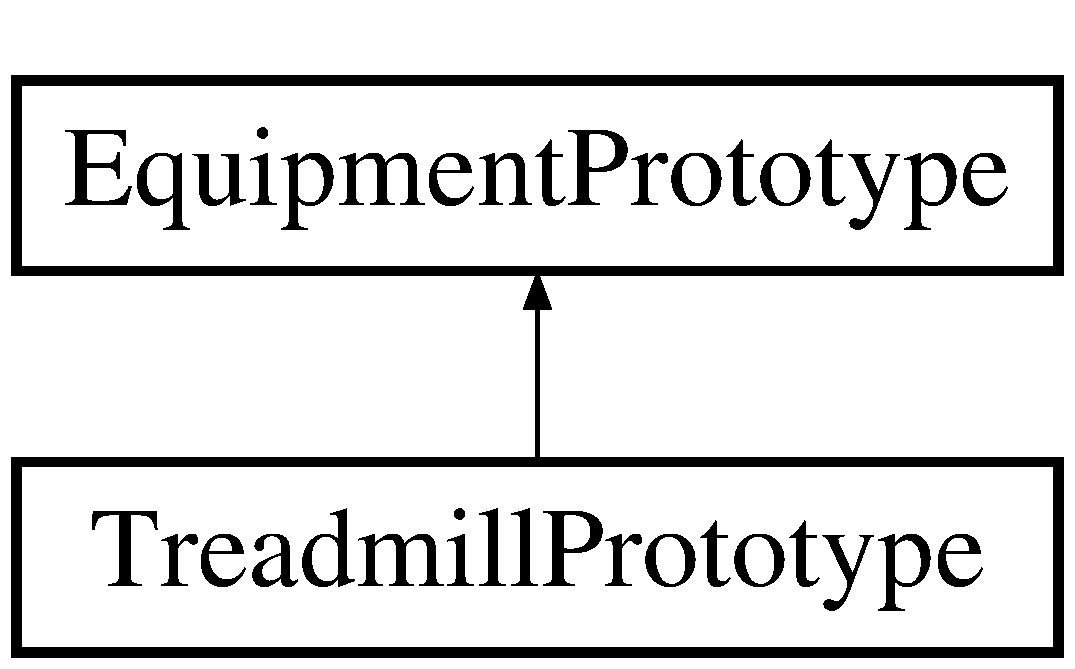
\includegraphics[height=2.000000cm]{class_treadmill_prototype}
\end{center}
\end{figure}
\subsection*{Public Member Functions}
\begin{DoxyCompactItemize}
\item 
\hypertarget{class_treadmill_prototype_af0689fe2a2c25382690f38e7926d5721}{}\hyperlink{class_treadmill_prototype_af0689fe2a2c25382690f38e7926d5721}{Treadmill\+Prototype} ()\label{class_treadmill_prototype_af0689fe2a2c25382690f38e7926d5721}

\begin{DoxyCompactList}\small\item\em Constructor. \end{DoxyCompactList}\item 
\hypertarget{class_treadmill_prototype_aa26e5b7c3dcf15d9c7fc59e621f77e5c}{}\hyperlink{class_treadmill_prototype_aa26e5b7c3dcf15d9c7fc59e621f77e5c}{Treadmill\+Prototype} (const \hyperlink{class_treadmill_prototype}{Treadmill\+Prototype} \&)\label{class_treadmill_prototype_aa26e5b7c3dcf15d9c7fc59e621f77e5c}

\begin{DoxyCompactList}\small\item\em Copy Constructor. \end{DoxyCompactList}\item 
\hyperlink{class_equipment_prototype}{Equipment\+Prototype} $\ast$ \hyperlink{class_treadmill_prototype_abd7e7f894721af9f03b248b6617d4fdc}{clone} () const 
\begin{DoxyCompactList}\small\item\em Clone. \end{DoxyCompactList}\end{DoxyCompactItemize}
\subsection*{Additional Inherited Members}


\subsection{Detailed Description}
\hyperlink{class_treadmill_prototype}{Treadmill\+Prototype} Class. 

Used for holding information regarding a treadmill 

\subsection{Member Function Documentation}
\hypertarget{class_treadmill_prototype_abd7e7f894721af9f03b248b6617d4fdc}{}\index{Treadmill\+Prototype@{Treadmill\+Prototype}!clone@{clone}}
\index{clone@{clone}!Treadmill\+Prototype@{Treadmill\+Prototype}}
\subsubsection[{clone() const }]{\setlength{\rightskip}{0pt plus 5cm}{\bf Equipment\+Prototype} $\ast$ Treadmill\+Prototype\+::clone (
\begin{DoxyParamCaption}
{}
\end{DoxyParamCaption}
) const\hspace{0.3cm}{\ttfamily [virtual]}}\label{class_treadmill_prototype_abd7e7f894721af9f03b248b6617d4fdc}


Clone. 

Returns a pointer to a new \hyperlink{class_treadmill_prototype}{Treadmill\+Prototype} object that is identical to this one. 

Implements \hyperlink{class_equipment_prototype_a4014d69b92c71c4c49477c657c824024}{Equipment\+Prototype}.



The documentation for this class was generated from the following files\+:\begin{DoxyCompactItemize}
\item 
/\+Users/jshier/\+Development/\+Exercise\+Software/\+Exercise\+Software/treadmill\+\_\+prototype.\+hpp\item 
/\+Users/jshier/\+Development/\+Exercise\+Software/\+Exercise\+Software/treadmill\+\_\+prototype.\+cpp\end{DoxyCompactItemize}

%--- End generated contents ---

% Index
\backmatter
\newpage
\phantomsection
\clearemptydoublepage
\addcontentsline{toc}{chapter}{Index}
\printindex

\end{document}
